\scanpage{20}
% @ upper left, letterhead
% letterhead
M. DUFOUR\\
VARITYPISTE\\
131, \textsc{Rue Lecourbe}\\
PARIS XV\textsuperscript{e}\\
$\blacksquare$\\
C. C. P. Paris 14.143-34\\
R. M. 140.029

% @ 1–3, at the head and right of the letterhead
\uline{Lemme} \unsure{!}
Si $X\xrightarrow{f}Y$ admet une section \deleted{\unsure{$s$}}$s$, alors $s(Y)$ est à la fois \deleted{\unsure{ouvert}} \uline{fermé} et \uuline{ouvert}. En effet,

% @ left margin, beside 4–6
\margin{\figure{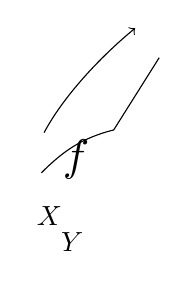
\begin{tikzpicture}[x=.34cm,y=.34cm]
\draw[thin,->] (.2,3.0) .. controls (1,4.5) and (2.5,6.0) .. (3.6,6.9);
\draw[thin] (.1,1.5) .. controls (.9,2.3) and (1.6,2.8) .. (2.8,3.1) -- (4.5,5.8);
\node[scale=1.6] at (1.4,2.0) {$\unsure{f}$};
\node at (.4,-.1) {$X$}; \node at (1.25,-1.1) {$Y$};
\end{tikzpicture}}}

% @ 4–11, heavily cancelled central argument
\deleted{on voit de suite que c'est une réunion $X'$ de composantes irréductibles de $X$ [$X\to Y$ est fini] il faut montrer que si \deleted{\unsure{une}} $X''$ est \deleted{une} la réunion des autres composantes irréductibles, alors $X'\cap X''=\varnothing$. Or \deleted{\unsure{on a que}} \unsure{générique de|qu'en un pt de|l'image} \unsure{une|un} composante de $Y$, on \unsure{$\nu''(y)=n-1$|$d''(y)=n-1$}, donc les composantes irréductibles de}

% @ 12–16, under the cancelled argument
Pour ce dernier point on est ramené au cas où $Y$ est irréductible [car si les $Y_i$ sont les composantes de $Y$, il suffit de prouver que $s(\unsure{y|Y|Y_i})$ induit un ouvert sur chaque $f^{-1}(\unsure{Y|Y_i})$], or alors les composantes irréductibles de $X$ sont \uline{disjointes} [\unsure{vif|vérif}], \unsure{en} \deleted{\unsure{par exemple}} d'où la conclusion.

% @ left margin, level with the reduction to components
\margin{\diagram{\begin{tikzcd}[ampersand replacement=\&,column sep=tiny,row sep=small]
X\arrow[d]\&\deleted{\unsure{=X}}\displaystyle\bigcup_i f^{-1}(Y_i)\arrow[d] \\
Y\arrow[u,bend left=35,"s"]\&{}=\displaystyle\bigcup_i Y_i\arrow[u,bend left=35,"s_i"]
\end{tikzcd}}}

% @ 17–18, foot
Donc on aura $X=X_{(1)}\amalg X^{(1)}$, où $\unsure{\nu|v|d}(X_{(1)}/Y)=1$, $\nu(X^{(1)}/Y)=n-1$.
% @ central sideways watermark
% printed form
% the paper's watermark (EXTRA STRONG), not his text
\unsure{Guerimand|Guérimand} Voiron
% archive sheet number: 19
